\documentclass[]{jsarticle}
\usepackage{bm}
\usepackage{braket}
\usepackage[dvipdfmx]{graphicx}
\usepackage{tikz}
\title{Laughlin}
\author{松本大輝}
\date{}

\begin{document}
\maketitle
%\section{Laughlinの議論}
%一定磁場下の二次元電子系ではランダウ準位という等間隔に離散化されたエネルギー準位が
%形成され、この準位間にフェルミエネルギーがあると系は絶縁体となる。このようなときに
%ホール伝導度が
Laughlinはゲージ不変性を用いてホール伝導度が量子化されることを説明した.このノートはそのLaughlinの議論
を個人的にまとめたものである.
図のようなシリンダー状の二次元電子系を考える.シリンダーの周長を$L_y$,高さを$L_x$とする.系の表面を一様な磁場$B_0$が垂直に貫いているとする.
この系では周方向に流れるホール電流$I_y$はシリンダーを通る表面に接しない磁束$\Phi$を断熱的\footnote{Aharonov-Borm位相がBerry位相であることから"adiabatic derivative"か?}に入れたことにより生じたと考えることができる.
\begin{center}
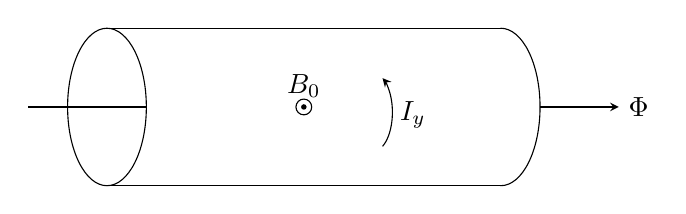
\begin{tikzpicture}
    \draw (5,0) circle[x radius=0.5,y radius=1];
    \draw (7.5,0)circle(0.1);
    \fill (7.5,0) circle(1pt);
    \draw (7.5,0) node[above]{$B_0$};
    \draw (10,-1) arc[start angle=-90, end angle=90 ,x radius = 0.5,y radius = 1];
    \draw (5,1)--(10,1);
    \draw (5,-1)--(10,-1);
    \draw (5.5,0)--(4,0);
    \draw (11.5,0) node[right]{$\Phi$};
    \draw [->,>=stealth](10.5,0)--(11.5,0);
    \draw [->,>=stealth](8.5,-0.5) arc[start angle=-60, end angle=60 ,x radius = 0.25,y radius = 0.5];
    \draw (8.6,-0.1) node[right]{$I_y$};
\end{tikzpicture}
\end{center}
この磁束により生じるベクトルポテンシャルの周方向の成分は磁束$\Phi$と
\begin{equation}
    \Phi = \int A_y dy = A_y L_y,
\end{equation}
という関係にある.これにより$\Phi$を入れた後の一電子ハミルトニアン
\begin{equation}
    H = \frac{1}{2m} \left(\bm{p} - \frac{e}{c}\bm{A} \right)^2,
\end{equation}
はパラメータ$\Phi$に依存することになる.今ホール電流は,電子の平均速度を$\bar{\braket{v_y}}$とすると
\begin{equation}
    I_y = -e\rho\bar{\braket{v_y}}L_x,
\end{equation}
と表される.ここで電子密度$\rho$は系の電子の総数が$N$個だとして$\rho = N/L_xL_y$である.一電子の速度の周方向の成分は,Hellmann-Feymnamの定理より,電子が固有状態$\ket{k}$にありエネルギー固有値が$E_k$
であったとすれば
\begin{equation}
    \frac{dE_k}{d\Phi} = \bra{k} \frac{dH}{d\Phi}\ket{k} = -\frac{e}{mcL_y}\bra{k} (p_y - \frac{e}{c} A_y)\ket{k} = -\frac{e}{cL_y}\braket{v_y},
\end{equation}
となり,電子の周方向の平均速度$\bar{\braket{v_y}}$は,
\begin{equation}
    \bar{\braket{v_y}} = \frac{1}{N} \sum \braket{v_y} = -\frac{cL_y}{e}\sum\frac{dE_k}{d\Phi} = -\frac{cL_y}{eN}\frac{dU}{d\Phi},
\end{equation}
と表せる.ここで$U$は電子系の全エネルギーである.(3),(5)式からホール電流$I_y$と全エネルギー$U$と磁束$\Phi$の関係式
\begin{equation}
    I_y = \frac{eNL_x}{L_xL_y} \frac{cL_y}{eN} \frac{dU}{d\Phi} = c\frac{dU}{d\Phi},
\end{equation}
が得られる.

ゲージ変換によって波動関数には$\exp{\left(\displaystyle \frac{ieA_y y}{c\hbar}\right)}$だけの位相が生じるが,
周方向の周期的境界条件を考慮すると,
\begin{eqnarray}
    \frac{eA_y}{c\hbar} L_y &=& 2n\pi \nonumber \\
    A_y &=& n \frac{hc}{e} \times \frac{1}{L_y}
\end{eqnarray}
これと(1)式より$\Phi = n(hc/e) $となり,シリンダーに入る磁束はモノポールの整数倍であるとわかる.ここでは,系に入れる磁束を
$\Phi = hc/e$とする.

次に具体的にハミルトニアンを見てみる.ランダウゲージ$\bm{A} = (0,B_0x,0)$を採用すれば,磁束を入れる前の系のハミルトニアンは
\begin{equation}
    H = \frac{1}{2m}\left\{p_x^2 + \left(p_y - \frac{eB_0x}{c} \right)^2 \right \},
\end{equation}
である.ハミルトニアンが$y$を含まないため$[H,p_y] = 0$であり,$p_y$の固有値を$\hbar k_y$とすれば
\begin{equation}
    H = \frac{1}{2m} p_x^2  + \frac{m}{2} \omega^2 \left(x - \frac{c \hbar k_y}{eB_0} \right)^2,
\end{equation}
$\omega = eB_0/mc$は振動数,$x_0 = c\hbar k_y /eB_0$は振動中心である.これは調和振動子のハミルトニアンであり,したがって系のエネルギー準位は
\begin{equation}
    E_n = \hbar \omega \left(n + \frac{1}{2} \right),
\end{equation}
と離散的に量子化されたランダウ準位となる.

磁束が入った後もゲージ不変性によりハミルトニアン自体は不変であり,エネルギー分散も変化しない.しかし,元の系の波動関数を$e^{ik_y y}\phi_n$とすれば,
磁束を入れることにより波動関数は$e^{ik_y y} \phi_n \to e^{i(k_y + eA_y /\hbar c)y} \phi_n $ と変化するため,磁束が入ると振動中心が
$\displaystyle x_0 \to x_0 + \frac{A_y}{B_0} $だけズレる.すなわち,系の電子が$x$方向に移動する.
系の左端から右端の電位差が$V$であり,磁束を入れる前後で$n$個の電子が端から端まで移動したとする.そうすると系の全エネルギーの変化$\Delta U$は$\Delta U = neV$
となる.$\displaystyle \frac{dU}{d\Phi} \to \frac{\Delta U}{ \Delta \Phi}$という置き換え\footnote{磁束の変化が磁束量子分であることから,微分を差分に置き換える近似が正当化されているか.}によりホール電流は
\begin{equation}
    I_y = c\frac{\Delta U}{\Delta \Phi} = c\frac{neV}{hc/e} = n \frac{e^2}{h} V
\end{equation}
となる.したがってホール伝導度$\sigma_{xy}$は
\begin{equation}
    \sigma_{xy} = -\sigma_{yx} = \frac{I_y}{V} = -n\frac{e^2}{h}
\end{equation}
と,$e^2/h$を単位とした整数値をとる.

%\section{付録}
%\subsection{ゲージ変換}
%\subsection{Aharonov-Bohm効果}
\end{document}